\documentclass{article}
\usepackage[utf8]{inputenc}
\usepackage[margin=1in]{geometry}
\usepackage{xcolor, tikz, amsmath, amssymb, amsthm, fancyhdr, xfrac, physics, cleveref}

%\pagecolor[rgb]{0.2,0.2,0.2}
%\color[rgb]{1,1,1}

% Headers
\pagestyle{fancy}
\fancyhf{}
\rhead{Max Ortner}
\lhead{Calculus III}
\chead{Problem Set I}
\cfoot{Page \thepage}
\renewcommand{\headrulewidth}{0pt}
\renewcommand{\footrulewidth}{0pt}

\newcommand{\nhat}[1]{\boldsymbol{\hat{\textbf{#1}}}}

\newcommand{\qnumber}[1]{
\vspace{0.5cm}
\noindent
\textbf{#1.}
\vspace{4mm}
}

\setlength{\parskip}{0.15cm}
%\setlength{\parindent}{0em}
\renewcommand{\baselinestretch}{1.2}

\newtheorem{theorem}{Theorem}
\newtheorem{post}{Postulate}

\begin{document}

%\begin{flushright}
%    Max Ortner
%\end{flushright}

\begin{center}
    \huge Calculus III
    
    \large Problem Set I

    \normalsize Max Ortner
    \thispagestyle{plain}
\end{center}



\qnumber{1}

\noindent
Let there exist three vectors $\vec{r}=\langle x, y, z \rangle$, $\vec{a}=\langle a_1, a_2, a_3 \rangle$, and $\vec{b}=\langle b_1, b_2, b_3 \rangle$. Consider the set of vectors $S$, where $\vec{r}\in S$, that satisfy
\[
    (\vec{r}-\vec{a}) \cdot (\vec{r}-\vec{b})=0.
\]
To get this into a more understandable form, let us expand it algebraically. Because of the distributive property of the dot-product, we can distribute it throughout each term and replace the vector's with their components to get
\[
    x^2+y^2+z^2 - (xa_1 + ya_2 + za_3) - (xb_1 + yb_2 + zb_3) + a_1b_1 + a_2b_2 + a_3b_3=0.
\]
Having each component of $\vec{r}$ on the left side multiplied by itself and added together is a major piece of evidence that this equation represents a sphere. We can group together the variables and subtract each side by the terms equivalent to $\vec{a}\cdot\vec{b}$.

Think about only the $x$-component of this expression, namely
\[
    x^2-x(a_1+b_1).  
\]
To factor this expression we can equate it to 0 and complete the square:
\[
    x^2-x(a_1+b_1) + \frac{(a_1+b_1)^2}{4} = \frac{(a_1+b_1)^2}{4} = \left( x - \frac{1}{2}(a_1+b_1) \right)^2.
\]
We can follow this procedure for each variable and accrue their completed square quantity to get
\[
\begin{split}
    \left( x - \frac{1}{2}(a_1+b_1) \right)^2 + &\left( y - \frac{1}{2}(a_2+b_2) \right)^2 + \left( z - \frac{1}{2}(a_3+b_3) \right)^2 \\
    &=-(\vec{a}\cdot\vec{b})+\frac{(a_1+b_1)^2}{4}+\frac{(a_2+b_2)^2}{4}+\frac{(a_3+b_3)^2}{4}.
\end{split}
\]
It is evident, even before pursuing simplification, the origin point of the circle is $\frac{1}{2}(\vec{a}+\vec{b})$. Expanding each of the terms on the right side and combining with the component version of $-(\vec{a}\cdot\vec{b})$ simplifies the expression significantly. Thus, taking the square root of the right side after simplifying gives, for the radius $r$,
\[
    r=\frac{|\vec{a}-\vec{b}|}{2}.
\]

\qnumber{2}

\noindent
Consider a cube in three-space. The diagonal connecting the origin to the furthest point can be described as a vector
\begin{equation} \label{eq:cube_diagonal}
    \vec{L}=c\:\langle 1, 1, 1 \rangle,
\end{equation}
where $c$ is the length of the sides of the cube. Although a cube has six sides, there are only three unique face diagonals. Each face has a side opposite it which has equivalent diagonals, and the face diagonals in the other direction are simply reflections across the origin. 

Therefore, the set of distinct face diagonals $S$ has as its elements $\vec{s}_n,\;n\in\{1, 2, 3\}$. Thus
\[
\begin{split}
    \vec{s}_1 &= c\:\langle 0, 1, 1 \rangle, \\
    \vec{s}_2 &= c\:\langle 1, 0, 1 \rangle, \\
    \vec{s}_3 &= c\:\langle 1, 1, 0 \rangle.
\end{split}  
\]
Before considering a theorem for this explicitly defined set, let us first establish two fundamental postulates used to relate each of its elements.
\begin{post} \label{post:sum_n}
    For any choice of $n$, the sum of the components is equivalent to any other choice of $n$.
\end{post}
\begin{post} \label{post:magnitude}
    Since the magnitude of every non-zero component of $\vec{s}_n$ is $c$, and since every $\vec{s}_n$ contains only two non-zero components, the magnitude of $\vec{s}_n$ is equivalent to every other choice of $n$ in the set.
\end{post}
\noindent
With these self-evident properties established, let us form a theorem.

\begin{quote}
\begin{theorem} \label{thm:scalar_product}
    Given a set of distinct diagonals each associated with a face of a cube, the scalar products between the diagonal of the cube and each of these vectors are equivalent.
\end{theorem}

\begin{proof}
    %Let $\vec{s}_n\in S$ and $n\in\{1, 2, 3\}$. For every $n$, the sum of each component of the vector $\vec{s}_n$, namely $\Sigma \vec{s}_n$, can be found to be\footnote{\textit{Although I don't particularly enjoy computing the sum of the components of each element of the set explicitly, I guess since the set itself is explicitly defined rather than formulaically, there isn't a more general way to do it (or is there\dots).}}
    %\[
    %\begin{split}
    %    \Sigma \vec{s}_1 &= 2c, \\
    %    \Sigma \vec{s}_2 &= 2c, \\
    %    \Sigma \vec{s}_3 &= 2c.
    %\end{split}
    %\]
    
    %Let us also define the dot product of the cube diagonal, $\vec{L}$, with an arbitrary three-dimensional vector $\vec{v}$ as

    Let there exist an arbitrary vector in three-space $\vec{v}$, and let the distinct cube diagonal be $\vec{L}$ as defined in equation \ref{eq:cube_diagonal}. Consider the scalar-product between these vectors,
    \[
        \vec{v} \cdot \vec{L} = c( \vec{v}_x + \vec{v}_y + \vec{v}_z ).
    \]
    With this, it is apparent that $\vec{v} \cdot \vec{L} = c\,\Sigma \vec{v}$, where $\Sigma \vec{v}$ denotes the sum of the components of $\vec{v}$. Since the dot-product of any vector with the cube diagonal $\vec{L}$ relies only upon the sum of the components of the arbitrary vector, it follows that two independent vectors who share only the sum of their components would give an equivalent result when producing a scalar product with $\vec{L}$. 
    
    Therefore, from the conclusion of postulate \ref{post:sum_n}, all vectors in this set when multiplied with $\vec{L}$ produce the same result.
\end{proof}
\end{quote}

We can find the angle formed between the cube diagonal and an arbitrary face-diagonal by considering the definition of $\cos\theta$ with relation to two vector's dot product, namely
\[
    \cos\theta = \frac{\vec{L} \cdot \vec{s}_n}{|\vec{L}|\,|\vec{s}_n|}.  
\]
As shown in theorem \ref{thm:scalar_product}, the numerator can be simplified to
\[
    \vec{L} \cdot \vec{s}_n = c\Sigma \vec{s}_n = 2c^2.
\]
The magnitude of the face diagonal can be computed to be $c\sqrt{3}$. Because of postulate \ref{post:magnitude}, we need only find one of the magnitudes of the face-diagonals. It can easily be found to be $c\sqrt{2}$. Now we have all the information to construct the angle:
\[
    \cos\theta = \frac{2c^2}{c^2\sqrt{6}}  = \frac{2}{\sqrt{6}}.
\]
Solving for $\theta$ gives an angle of approximately $35.3^\circ$.

\qnumber{3}

\begin{figure}[h]
    \centering

    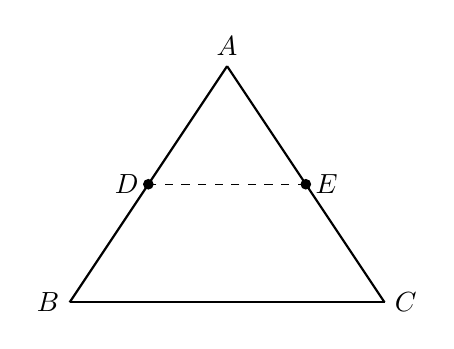
\begin{tikzpicture}[scale=2]
        \draw[thick] (0, 1.5) -- (-1, 0) node[left] {$B$}; 
        \draw[thick] (-1, 0)  -- (1, 0) node[right] {$C$};
        \draw[thick] ( 1, 0)  -- (0, 1.5) node[above] {$A$};

        \draw[fill] ( 0.5, 0.75) circle (0.03) node[right] {$E$};
        \draw[fill] (-0.5, 0.75) circle (0.03) node[left]  {$D$};

        \draw[dashed] ( 0.5, 0.75 ) -- ( -0.5, 0.75 );
    \end{tikzpicture}

\end{figure}

\noindent
Let there exist a triangle $ABC$. Consider the vector $\vec{a}$ connecting the points $BC$, where $B$ is the initial point and $C$ is the terminal point. If each vertex is a position vector,
\[
    \vec{a}=\vec{C}-\vec{B}.  
\] 
The midpoint of the lines $AB$ and $AC$ (again when considering the vertices as position vectors) are $\frac{1}{2}(\vec{B}-\vec{A})$ and $\frac{1}{2}(\vec{C}-\vec{A})$. These represent the points $D$ and $E$ on the graphic, respectively. The line that joins the midpoints, $\vec{m}$, is $\vec{E} - \vec{D}$ or,
\[
    \vec{m}=\frac{1}{2}(\vec{C}-\vec{A} -\vec{B} + \vec{A} )=\frac{1}{2}\vec{a}.
\]
Therefore, the line between the base and a corner connecting the midpoints of the other two lines of a triangle is exactly one half the vector of the base.

We can determine whether or not the base and the mid-line are parallel by considering the angle between them. Given that $\vec{m}$ is defined in terms of a scalar multiple of $\vec{a}$ it is evident they share the same unit vector (or direction), i.e. $\hat{m}=\hat{a}$. We can use this fact to determine $\cos\theta$ where $\theta$ is the angle between them by utilizing the relationship between unit vectors and $\cos\theta$ shown in equation \ref{eq:cos} on page \pageref{eq:cos},
\[
    \cos\theta=\hat{m} \cdot \hat{a}=|\hat{m}|^2=1.
\]
Solving for $\theta$ gives $\theta=0$ (assuming multiples of $2\pi$ are reduced back down to 0) which means they are parallel.

\qnumber{4}

\noindent
Consider the interaction required to change the course of a plane flying north at 180 $\sfrac{\text{km}}{\text{hr}}$. The plane takes off moving at this rate. After one half of an hour has passed, the distance travelled is actually 80 km at 5$^\circ$ east of north. Since the velocity is given as distance travelled per hour passed, the total distance travelled by the original velocity in one hour \emph{would be} 180 km. To find the average velocity of the plane over its course, we need to consider the distance it \emph{actually} travelled in one hour. 


Let's first think about the displacement vector, $\vec{d}$. The direction of 5$^\circ$ east of north relates sine to the $x$-component and cosine to the $y$-component, and 80 is its magnitude. Also, since east of north is in the first quadrant, all components are positive. Therefore,
\[
    \vec{d}=80\langle \sin 5^\circ, \cos 5^\circ \rangle.
\]
If the change in time, $\Delta t$, is given in hours, $\Delta t = \frac{1}{2}$. Thus to find the average velocity we multiply $\frac{1}{\Delta t}$ to $\vec{d}$ getting
\[
    \vec{v}=160\langle \sin 5^\circ, \cos 5^\circ \rangle.
\]
The only interaction that occurred that changed the planes course from its original trajectory was the wind, which is represented by the vector $\vec{w}$. The resultant velocity $\vec{v}$ represents the velocity of the plane after the wind had interacted with its given initial velocity, $\vec{v}_i$. This relationship can be described as
\[
    \vec{v}=\vec{w}+\vec{v}_i.  
\]
To find $\vec{w}$, we must simply subtract $\vec{v}_i$ from $\vec{v}$. Or, since we know $\vec{v}_i$ to be 180 $\sfrac{\text{km}}{\text{hr}}$ north,
\[
\begin{split}
    \vec{w}&=160\langle \sin 5^\circ, \cos 5^\circ \rangle - \langle 0, 180 \rangle, \\
           &=20\langle 8 \sin 5^\circ, 8\cos 5^\circ - 9 \rangle.
\end{split}
\]

To determine the direction the pilot should have headed to reach the right direction, we need to know the vector such that when $\vec{w}$ is added to it, $\vec{v}_i$ is yielded. This vector, $\vec{n}$, must satisfy the property,
\[
    \vec{v}_i=\vec{w}+\vec{n}.
\]
Therefore, we can subtract from $\vec{v}_i$ the wind vector $\vec{w}$ to get\footnote{\textit{This result can easily be verified by considering the addition of this vector with the wind velocity vector $\vec{w}$, which yields $\langle 0, 180 \rangle$.}}
\[
\begin{split}
    \vec{n}&=20\langle 0, 9 \rangle - 20\langle 8 \sin 5^\circ, 8\cos 5^\circ - 9 \rangle, \\
           &=20\langle -8 \sin 5^\circ, -8 \cos 5^\circ + 18 \rangle.
\end{split}
\]
If we consider only the direction of this vector, we must find the unit vector, $\hat{n}$. To do this, we first must find the magnitude:
\[
    |\vec{n}|=\sqrt{64\sin^2 5^\circ + (8\cos 5^\circ + 18)^2}  
\]
Dividing $\vec{n}$ by this magnitude yields a large and unsatisfying unit vector. The angle can easily be computed by taking the inverse cosine of the $\frac{\vec{n}_x}{|\vec{n}|}$, which gives about $1.54^\circ$ west of north.

\qnumber{5} \footnote{\textit{I know this is all five problems, but I saw this and couldn't resist.}}

\begin{figure}[h]
    \centering

    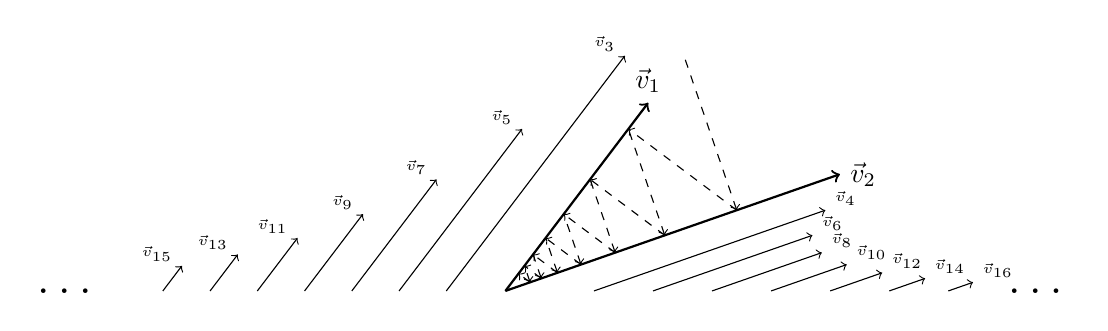
\begin{tikzpicture}[scale=1.5]
        \draw[->, thick] (0, 0) -- ( 0.9442 * 3.0, 0.32942 * 3.0) node[right] {$\vec{v}_2$};
        \draw[->, thick] (0, 0) -- (0.60473 * 2.0, 0.79643 * 2.0) node[left, above]  {$\vec{v}_1$};

        % Unit vector v_2
        \foreach \i in {1, 3, 5, 7, ..., 13} {
            \pgfmathsetmacro\result{\i + 3}
            \draw[->] (\i/4 + 1/2, 0) -- ( 0.9442 * 2.5 * 0.83^\i + \i/4 + 1/2, 0.32942 * 2.5 * 0.83^\i) node[above=0.15cm, right] {\tiny$\vec{v}_{\pgfmathprintnumber{\result}}$};
            
            \draw[->, dashed] ( 0.9442 * 2.5 * 0.83^\i, 0.32942 * 2.5 * 0.83^\i) -- (0.60473 * 0.83 * 2.5 * 0.83^\i, 0.79643 * 2.5 * 0.83 * 0.83^\i);
        }
        
        % Unit vector v_1
        \foreach \i in {0, 2, 4, 6, ..., 12} {
            \pgfmathsetmacro\result{\i + 3}
            \draw[->] (-\i/5 - 1/2, 0) -- (0.60473 * 2.5 * 0.83^\i - \i/5 - 1/2, 0.79643 * 2.5 * 0.83^\i) node[above=0.15cm, left] {\tiny$\vec{v}_{\pgfmathprintnumber{\result}}$};
            
            \draw[<-, dashed] ( 0.9442 * 2.5 * 0.83 * 0.83^\i, 0.32942 * 2.5 * 0.83 * 0.83^\i) -- (0.60473 * 2.5 * 0.83^\i, 0.79643 * 2.5 * 0.83^\i);
        }

        \node[draw=none] at ( 4.52, 0) {\LARGE$\dots$};
        \node[draw=none] at (-3.7, 0) {\LARGE$\dots$};

    \end{tikzpicture}

    \caption{Diagram of the vectors constructed by equation \ref{eq:set_def}.}

\end{figure}

\noindent
Let there exist a set of vectors $V=\left\{ \vec{v}_1,\,\vec{v}_2,\,\dots \right\}$ and $\vec{v}_n\in V$, where $n\in Z^+$. Let $|\vec{v}_1|=2$, $|\vec{v}_2|=3$, and $\vec{v}_1\cdot\vec{v}_2=5$. For all $n>2$,
\begin{equation} \label{eq:set_def}
    \vec{v}_n=\text{proj}_{\vec{v}_{n-2}}\,\vec{v}_{n-1}.
\end{equation}

\begin{quote}
\begin{theorem} \label{thm:first}
Any vector $\vec{a}\in V$ holds the property that either $\hat{a}=\hat{v}_1$ or $\hat{a}=\hat{v}_2$, where $\hat{a}$ represents the unit vector of $\vec{a}$.
\end{theorem}

\begin{proof}
Let $\vec{v}_n\in V$ where $n\in \mathbb{Z}^+$ and $n>2$. By expanding the definition of a projection in equation \ref{eq:set_def}, we can obtain
\[
    \vec{v}_n=\frac{\vec{v}_{n-2}\cdot\vec{v}_{n-1}}{|\vec{v}_{n-2}|}\left(\frac{\vec{v}_{n-2}}{|\vec{v}_{n-2}|}\right).
\]
Since $\vec{v}_{n-2}$ is being divided by its magnitude in the parenthesis, it is the unit vector in that direction. Because of this, the unit vector of the left hand expression can be written as $\hat{v}$, and the unit vector of the right hand expression would be the rational term within the parenthesis. Symbolically,
\[
    \hat{v}_n=\frac{\vec{v}_{n-2}}{|\vec{v}_{n-2}|}=\hat{v}_{n-2}.
\]
Therefore,
\[
    \hat{v}_n=\hat{v}_{n-2}=\hat{v}_{n-4}=\dots
\]
Since the indices are only well-defined for values greater than $0$, $n-2k\geq1$, where $k\in \mathbb{Z}^+$. When $n$ is even, $n-2k=2$, and when $n$ is odd, $n-2k=1$. Therefore, for any choice of $n$, $\hat{v}_n$ is either $\hat{v}_1$ or $\hat{v}_2$.

\end{proof}
\end{quote}

Consider the relationship between two vectors $\vec{v}_n,\, \vec{v}_{n-1} \in V$,
\begin{equation} \label{eq:cos}
    \cos\theta = \frac{ \vec{v}_n \cdot \vec{v}_{n-1} }{ |\vec{v}_n|\:|\vec{v}_{n-1}| } = \left(\frac{\vec{v}_n}{|\vec{v}_n|}\right) \cdot \left(\frac{\vec{v}_{n-1}}{|\vec{v}_{n-1}|}\right)=\hat{v}_n \cdot \hat{v}_{n-1}.
\end{equation}
Because of the commutative property of the scalar product of two vectors, the order by which each unit vector is multiplied does not matter. Also, theorem \ref{thm:first} shows that, since if $n$ is even, $n-1$ is odd or vice versa, the ill-defined previous equation can be written as
\begin{equation} \label{eq:dotprod1}
    \hat{v}_n \cdot \hat{v}_{n-1} = \hat{v}_1 \cdot \hat{v}_2.
\end{equation}

Consider again the definition of the set for $n>2$ in equation \ref{eq:set_def}. The magnitude of $|\vec{v}_n|$ is the scalar on the right hand side of the equation being multiplied by the unit vector. We expand that equation with the definition of a projection and equate the magnitude of either side:
\[
    |\vec{v}_n|=\frac{\vec{v}_{n-2} \cdot \vec{v}_{n-1}}{|\vec{v}_{n-2}|}=|\vec{v}_{n-1}|\cos\theta.
\]
The relationship shown in equations \ref{eq:cos} and \ref{eq:dotprod1} allow us to rewrite this equation as
\[
    |\vec{v}_n|=|\vec{v}_{n-1}|(\hat{v}_1 \cdot \hat{v}_2).
\] 
This demonstrates an intimate relation between each subsequent vector's magnitude with the previous vector's magnitude. We can quantitively define $\cos\theta$ with the given information and the definition of the dot product in terms of an angle,
\[
    \cos\theta=\frac{\vec{v}_1\cdot\vec{v}_2}{|\vec{v}_1|\:|\vec{v}_2|}=\frac{5}{6}.
\]
We have already found in equation \ref{eq:dotprod1} that this quantity is equal to the dot product between the base unit vectors. Now we can describe $|\vec{v}_n|$ in terms of a ratio
\[
    |\vec{v}_n|=\frac{5}{6}|\vec{v}_{n-1}|.
\]

In order to define this explicitly we need a base case. In the current situation, the base case is when $n=3$. We can solve for $|\vec{v}_3|$ as
\[
    |\vec{v}_3|=\frac{5}{6}|\vec{v}_2|=\frac{5}{2}.
\]
Now we can construct $|\vec{v}_n|$ as a geometric sequence with the base value being $\frac{5}{2}$ and the ratio being $\frac{5}{6}$ to get
\[
    |\vec{v}_n|=\frac{5}{2}\left(\frac{5}{6}\right)^{n-3}. %=\frac{108}{25}\left(\frac{5}{6}\right)^n.
\]
To find the infinite sum of this expression, we must explicitly define the cases in which $n=1$ and $n=2$ and the rest using the sequence previously defined:
\[
    \sum_{n=1}^\infty |\vec{v}_n|=2+3+\frac{5}{2}\sum_{n=0}^\infty \left(\frac{5}{6}\right)^n.
\]
Since the sum of an infinite geometric series is known, we can substitute an expression in for the summation to get a quantifiable answer. This answer is
\[
    2+3+\frac{5}{2\left(1-\frac{5}{6}\right)}=20.
\]  
Therefore,
\[
    \sum_{n=1}^\infty |\vec{v}_n|=20.
\]

\vspace{2cm}

\noindent
Completed at: 5PM 9/4/2020

\noindent
Grade Received: ??

\end{document}